\chapter{Introduction}
\label{sec:introduction}

\section{Context} OK

In recent decades, the increasing adoption of industrial robotics has significantly
transformed manufacturing and automation processes. Modern production systems rely
on robots capable of performing complex tasks with high precision, repeatability,
and efficiency \cite{siciliano2009robotics}. At the same time, the integration of
machine vision technologies has enabled robots to perceive and interact with their
environment, leading to the development of vision-guided robotic systems for
applications such as object manipulation, quality inspection, and autonomous
assembly \cite{bradski2008learning}.

A key requirement for the correct operation of such systems is the ability to
accurately relate the coordinate frame of the vision sensor to the coordinate frame
of the robotic manipulator. In practice, poses and positions are expressed using
\textit{rigid body transformations}, represented as $4 \times 4$ homogeneous
transformation matrices of the form:

\begin{equation}
    \mathbf{T} = \begin{bmatrix} \mathbf{R} & \mathbf{t} \\ \mathbf{0}^{\top} & 1 \end{bmatrix}
    \in SE(3)
    \label{eq:homogeneous}
\end{equation}

\noindent where $\mathbf{R} \in SO(3)$ is a $3\times3$ rotation matrix and
$\mathbf{t} \in \mathbb{R}^3$ is a translation vector. The full set of such
matrices forms the Special Euclidean group $SE(3)$.

The process used to determine the rigid transformation between the camera and the
robot is commonly known as \textit{hand-eye calibration}
\cite{shiu1989calibration, tsai1989new}. This problem is fundamental in robot
vision, as it is required to correctly convert visual measurements, expressed in
the camera coordinate frame, into spatial commands that the robot can execute in
its own reference frame. Even small calibration errors can lead to significant
inaccuracies in positioning tasks, especially in applications requiring high
precision \cite{enebuse2021comparative}.

Various calibration approaches have been proposed in the literature, often
relying on the observation of calibration targets such as checkerboard patterns
or fiducial markers \cite{zhang2000flexible}. These methods typically involve
capturing multiple images of a known target while the robot moves through
different poses, allowing the estimation of the transformation between the robot
and camera coordinate frames. Despite the extensive research in this field,
practical implementation in industrial environments still presents several
challenges, including detection accuracy, measurement noise, and integration with
existing vision software tools \cite{enebuse2021comparative}.


\section{Motivation}

In modern industrial automation, many robotic systems rely on the integration of
machine vision to perform tasks such as object localization, inspection, and
manipulation. In these vision-guided robotic systems, it is essential to establish
an accurate spatial relationship between the camera and the robot—a relationship
determined through \textit{hand-eye calibration}
\cite{horaud1995hand, park1994robot}.

The accuracy of this calibration directly affects the performance of the overall
system. Calibration errors can propagate through the entire kinematic chain,
leading to positioning inaccuracies, manipulation failures, and reduced reliability
of automated processes \cite{enebuse2021comparative}. In industrial applications, where
precision and repeatability are critical, even small spatial misalignments can
significantly impact the effectiveness of robotic operations.

As the integration of vision systems in industrial robots becomes increasingly
widespread, there is a growing need for calibration procedures that are both
accurate and robust, while remaining practical to implement in real-world
environments. However, existing tools and software frameworks may present
limitations related to workflow efficiency, detection robustness, or ease of
integration \cite{enebuse2021comparative}. For these reasons, the development
and evaluation of reliable hand-eye calibration procedures remain an important
aspect in the deployment of vision-guided robotic systems.

Despite the extensive body of research on hand-eye calibration, the practical deployment of these methods in industrial environments remains challenging. Many existing approaches are primarily evaluated under controlled conditions and may exhibit limitations when integrated into real production systems, where factors such as measurement noise, detection robustness, and workflow constraints play a significant role.

In particular, issues related to the robustness of the calibration pipeline, the selection of suitable robot poses, and the seamless integration with existing vision software are often not fully addressed. These limitations highlight the need for calibration procedures that are not only theoretically sound, but also reliable and practical in real-world industrial applications.

This thesis addresses these challenges by developing and evaluating a complete hand-eye calibration workflow designed with a strong focus on robustness, integration, and experimental validation.


\section{Problem Statement}
\label{sec:problem_statement}

In vision-guided robotic systems, two main configurations exist depending on how
the camera is mounted with respect to the robot (see Figure~\ref{fig:hec_configs}):




\begin{itemize}
    \item \textbf{Eye-in-hand}: the camera is rigidly attached to the robot
    end-effector and moves with it. The unknown transformation $\mathbf{X}$
    relates the end-effector frame to the camera frame.

    \item \textbf{Eye-to-hand}: the camera is fixed in the environment and
    observes the robot workspace. The unknown transformation $\mathbf{X}$
    relates the robot base frame to the camera frame.
\end{itemize}

\begin{figure}[!htbp]
    \centering
    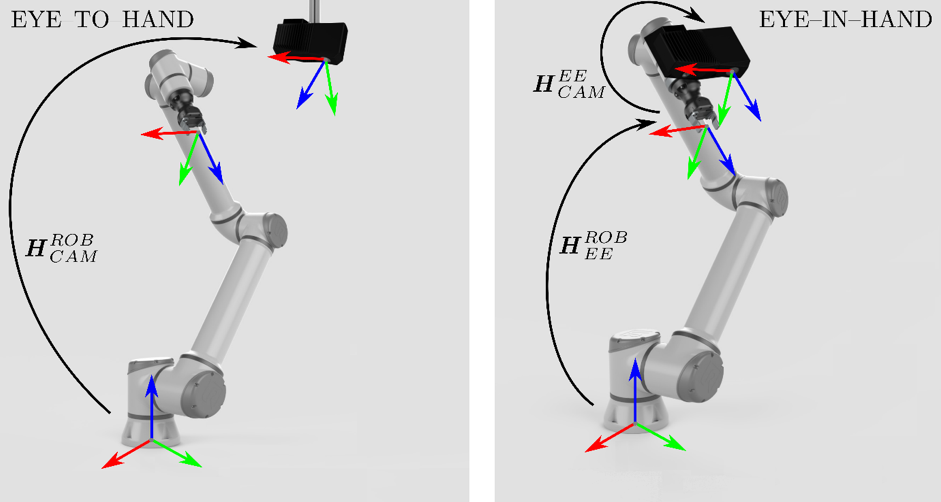
\includegraphics[width=0.7\textwidth]{images/chapter1Images/hand-eye-calib-configs.png}
    \caption{Eye-in-hand and eye-to-hand calibration configurations.}
    \label{fig:hec_configs}
\end{figure}

In both cases, by moving the robot through a set of $n$ distinct poses and
recording the corresponding camera observations, it is possible to formulate the hand-eye calibration problem as the matrix equation originally introduced by Shiu and Ahmad \cite{shiu1989calibration}:

\begin{equation}
    \mathbf{A}_i \mathbf{X} = \mathbf{X} \mathbf{B}_i, \qquad i = 1, \dots, n
    \label{eq:axb}
\end{equation}

\noindent where $\mathbf{A}_i \in SE(3)$ represents the relative motion of the
robot end-effector between pose $i$ and a reference pose, $\mathbf{B}_i \in SE(3)$
represents the corresponding relative motion of the calibration target as observed
by the camera, and $\mathbf{X} \in SE(3)$ is the unknown rigid transformation to
be estimated \cite{shiu1989calibration, tsai1989new}.

The matrix equation in \eqref{eq:axb} can be decomposed into its rotational and
translational components. Denoting $\mathbf{A}_i = (\mathbf{R}_{A_i},\,
\mathbf{t}_{A_i})$ and similarly for $\mathbf{B}_i$ and $\mathbf{X} =
(\mathbf{R}_X,\, \mathbf{t}_X)$, equation~\eqref{eq:axb} becomes:

\begin{align}
    \mathbf{R}_{A_i}\,\mathbf{R}_X &= \mathbf{R}_X\,\mathbf{R}_{B_i}
    \label{eq:rot_component}\\
    \mathbf{R}_{A_i}\,\mathbf{t}_X + \mathbf{t}_{A_i} &=
    \mathbf{R}_X\,\mathbf{t}_{B_i} + \mathbf{t}_X
    \label{eq:trans_component}
\end{align}

Several methods have been proposed to solve this system, including linear
decomposition approaches \cite{shiu1989calibration, tsai1989new}, methods based
on Lie group theory \cite{park1994robot}, and dual quaternion formulations
\cite{daniilidis1999hand} that solve for rotation and translation simultaneously.

However, obtaining an accurate and reliable estimate of $\mathbf{X}$ in practical
scenarios presents several challenges, including image quality, calibration target
detection accuracy, the choice and diversity of measurement poses, and the
robustness of the calibration pipeline within the vision software framework.

Therefore, the problem addressed in this thesis is the implementation and
evaluation of a hand-eye calibration workflow capable of estimating the
camera-to-robot transformation under both \textit{eye-in-hand} and
\textit{eye-to-hand} configurations, while considering the practical constraints
and potential sources of error that arise in real vision-guided robotic systems.
Furthermore, the developed pipeline includes a complete camera intrinsic calibration procedure, enabling a fully self-contained and camera-independent calibration workflow. This ensures that both intrinsic and extrinsic parameters can be estimated within a unified framework, improving flexibility and reproducibility in practical applications.




\section{Objectives}
\label{sec:objectives}

The main objective of this thesis is to design and evaluate a reliable hand-eye
calibration workflow for a vision-guided robotic system. In order to achieve this
goal, the following specific objectives are addressed:

\begin{itemize}
    \item Implement a complete hand-eye calibration pipeline capable of estimating
    the rigid transformation $\mathbf{X} \in SE(3)$ between the robot end-effector
    and the camera, supporting both eye-in-hand and eye-to-hand configurations.

    \item Integrate the calibration procedure within a machine vision framework
    used in the robotic system, ensuring compatibility with the existing vision
    tools and workflow.

    \item Evaluate different calibration algorithms and pose selection strategies
    in order to assess their performance and robustness in practical scenarios.

    \item Analyze potential sources of error in the calibration process, such as
    detection inaccuracies or measurement noise, with the aim of improving the
    reliability of the calibration results.

    \item Validate the calibration procedure through experimental tests, assessing
    the accuracy and consistency of the estimated transformation $\mathbf{X}$.
\end{itemize}


\section{Contribution}
\label{sec:contribution}

This thesis provides both methodological and practical contributions to the
field of hand-eye calibration in vision-guided robotic systems.

First, two distinct software solutions for hand-eye calibration have been
developed in different operational contexts.

The primary contribution consists in the design and implementation of a
complete eye-to-hand calibration module developed from scratch and
integrated within the software pipeline of an industrial SUPATA system
produced by EPF (Carrù, Italy). This solution is specifically tailored
for a production environment and operates exclusively in an eye-to-hand
configuration. The developed module replaces
previous calibration procedures that
showed limited robustness under
operational conditions,
providing improved reliability and consistency, and has been deployed on
a fully operational machine subsequently delivered to the end customer.

The second contribution consists in the development of a separate
calibration program implemented from scratch on a dedicated test bench.
In this setup, both \textit{eye-in-hand} and \textit{eye-to-hand}
configurations are supported. The system is not directly integrated with
the robot controller; instead, the robot is operated manually via the
teach pendant, while the calibration process relies on the robot-mounted
camera. This environment enables controlled experimentation, testing of
different calibration strategies, and validation of the proposed methods.

In addition to the implementation aspects, different calibration strategies
and pose acquisition procedures have been explored and compared. Tools for
performance evaluation have also been developed, including metrics based on
spatial consistency and error analysis, enabling a quantitative assessment
of calibration accuracy and robustness.

\section{Main Achievements}
\label{sec:achievements}

The main achievements of this thesis can be summarized as follows:

\begin{itemize}
	
	\item A complete camera intrinsic calibration
	procedure based on ChArUco targets was
	implemented and validated.
	
	\item A fully functional hand-eye calibration
	pipeline was developed and experimentally
	evaluated.
	
	\item An industrial eye-to-hand calibration
	module was integrated into a production-ready
	SUPATA system.
	
	\item Multiple hand-eye calibration algorithms
	were compared using identical datasets and
	evaluation metrics.
	
	\item Convergence analyses were performed to
	investigate the influence of dataset size and
	pose diversity.
	
	\item Quantitative metrics for calibration
	consistency and transformation stability
	were developed and applied.
	
\end{itemize}

\section{Significance of the Results}
\label{sec:significance}

The results obtained in this thesis have practical relevance for the deployment
of vision-guided robotic systems in industrial environments.

The proposed calibration workflow improves the reliability and accuracy of
camera-to-robot transformation estimation, which directly impacts the precision
of robotic operations such as inspection, localization, and manipulation.

The successful integration of the calibration module within an industrial
system demonstrates the feasibility of deploying robust calibration procedures
in real production environments, reducing the gap between theoretical methods
and practical implementation.

Furthermore, the availability of a dedicated test-bench setup enables systematic
evaluation and comparison of calibration strategies, providing useful insights
into the influence of different factors on calibration performance.

Overall, this work contributes to the development of more reliable and
reproducible calibration procedures, supporting the adoption of vision-guided
robotic systems in modern industrial applications.








%\section{Thesis Structure}
%\label{sec:structure}

% TODO: aggiorna questa sezione con la struttura reale della tua tesi.
%The remainder of this thesis is organized as follows:

%{itemize}
%    \item \textbf{Chapter~2} reviews the relevant literature on hand-eye
%    calibration methods and robot vision systems.
%    \item \textbf{Chapter~3} describes the mathematical background and the
%    calibration algorithms considered in this work.
%    \item \textbf{Chapter~4} presents the implementation of the calibration
%    pipeline and its integration within the vision framework.
%    \item \textbf{Chapter~5} reports the experimental results and discusses
%    the performance of the proposed approach.
%    \item \textbf{Chapter~6} draws conclusions and outlines possible directions
%    for future work.
%\end{itemize}